
\documentclass[11pt]{article}
% 11 point fonts

\usepackage{graphicx}
% for importing images

\usepackage{fixltx2e}
\usepackage{listings}
\usepackage{xcolor}
\lstset { %
    language=C++,
    backgroundcolor=\color{black!5}, % set backgroundcolor
    basicstyle=\footnotesize,% basic font setting
}

\usepackage[top = 1 in, bottom = 1 in, left = 0.75 in, right = 0.75 in]{geometry}
%margins

\begin{document}

\title{CS296 Report for Lab 5 and 6:\\
		Group 18}
	
\author{Rohit Kumar \\
		\textup{Roll No 120050028} \\
		\textit{rohit@cse.iitb.ac.in}
	\and
	Suman Sourabh \\
	\textup{Roll No 120050031} \\
	\textit{sumansourabh26@cse.iitb.ac.in}
	\and
	Nitin Chandrol\\
	\textup{Roll No 120050035} \\
	\textit{ntnchandrol@cse.iitb.ac.in}
	}

\date{\today}

\maketitle

\section{Introduction}

	\paragraph{}
	The purpose of this report is to explain the analyzed reports of timing experiments from Lab 5,
	 the effect of heavily loading a system while running the timing experiments 
	 by various kinds of programs like cpu heavy processes and memory heavy processes.
	 
	Further it explains the difference between \textbf{time} and \textbf{gettimeofday} using the observations that 
	we got.
	
	Finally we move to lab6 and compare the difference between the profiles created by debug profile 
	and by release profiles, study the effect of the level of optimization, i.e. \textbf{-On} option used while making the 
	executable using call graphs and profile data.

\section{Lab 5 Timing Experiments}
\paragraph{}
	
	\textit{Graph analysis-}

	Loop time increases with the number of iterations. As iteration number increases there will be more
	 number of 'for' loop execution and with each for loop initiating 150 steps. 
	Here gettimeoftheday is used for timing measurement and gettimeoftheday is called just before and after the for loop.

\begin{lstlisting}
gettimeofday(t1,null);

for(i=0;i<itr;i++){

//150 reruns

}

gettimeofday(t2,null);

\end{lstlisting}

Here, 	
\begin{itemize}
\item t = t2 - t1 is time for all processes running
\item y is the average time for each for loop execution
\item x is the time other system process takes while the code is running
\end{itemize}

\subsection{Plot 1 and 2 : Average time vs iteration values}
\paragraph{}
Average step time decreases with number of iteration and gets stabilized 
after some reruns.

\begin{equation}
	t_{step} = \frac {x+y*itr} {itr} = \frac {x} {itr} + y
\end{equation}


\begin{itemize}
\item Here, t\textsubscript{step}, the average step time is decreasing function of iteration value and for 
large value of iteration it gets stabilized.
\end{itemize}

Position update,velocity update and collision time shows similar nature like step time and gradually decreases with time.
Sum of all three update times contributes to a significant part of step time

These observations are clear from the following plot graphs:

\begin{center}
 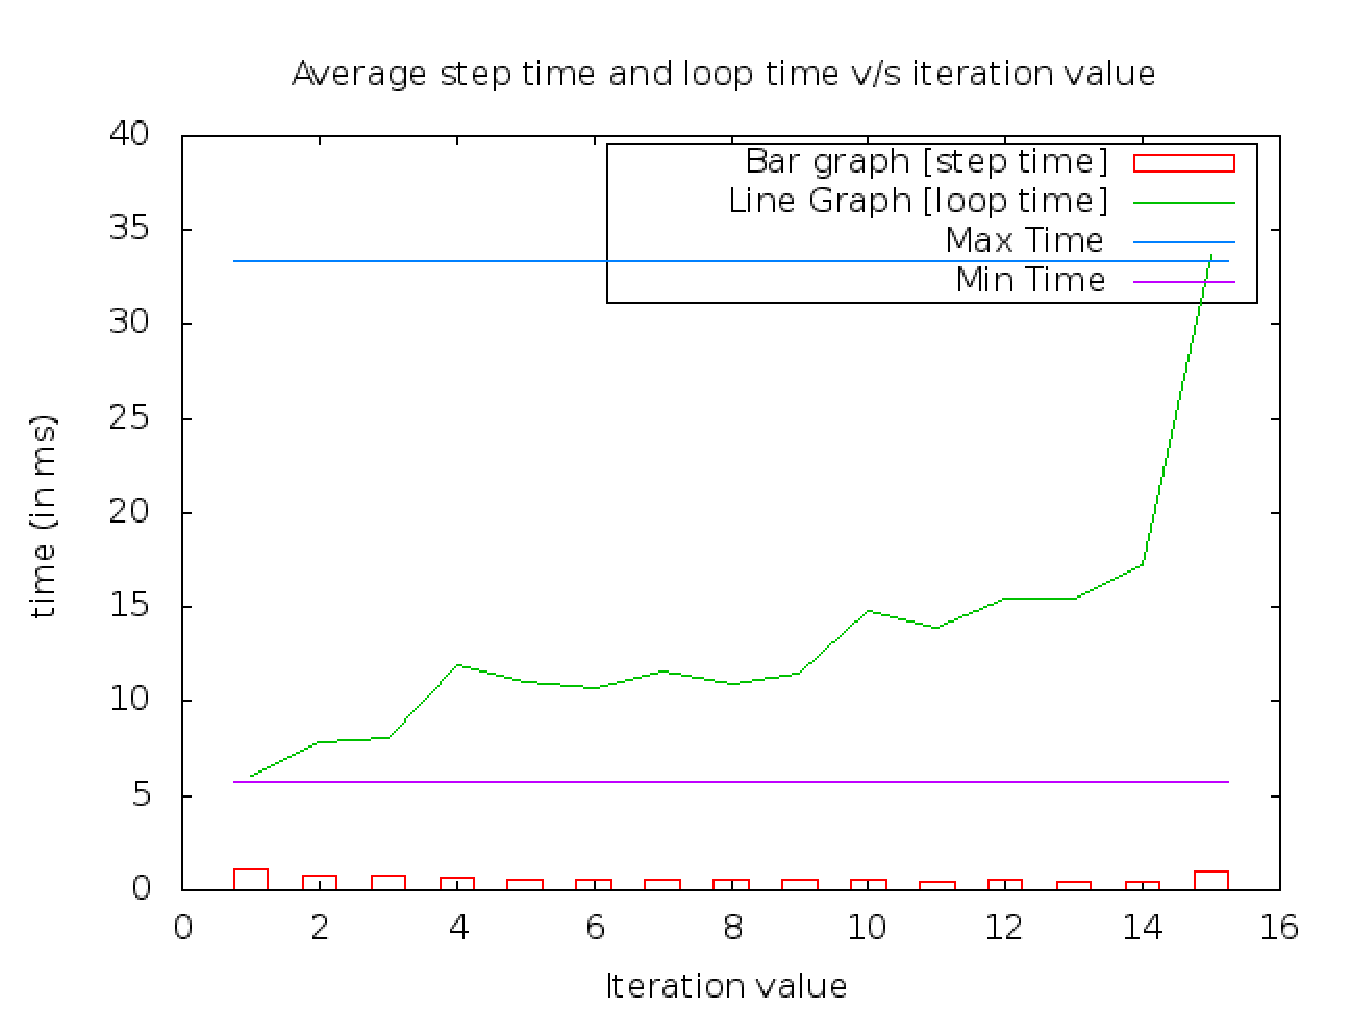
\includegraphics[scale = 0.4]{images/plot1} \\
  \emph{Average step time vs iteration values} \\
\end{center}

\begin{center}
 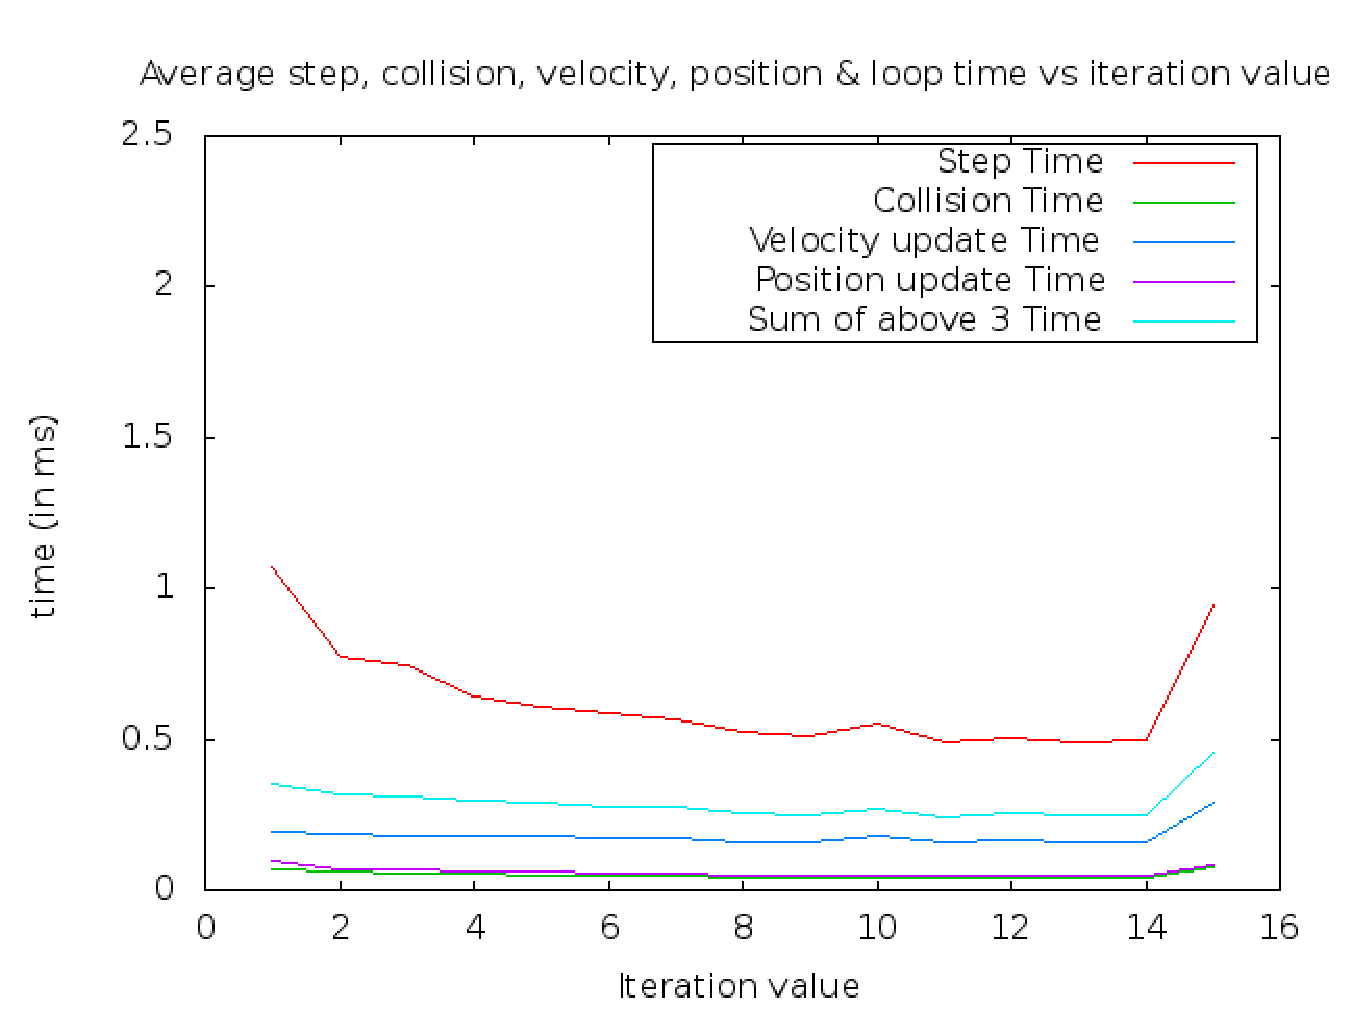
\includegraphics[scale = 0.4]{images/plot2} \\
  \emph{Average step, collision, velocity, position and loop time vs iteration value} \\
\end{center}

%%%%%%%%%%%%%%%%%%%%%%%%%%%%%%%%%%%%%%%%%%%%%%%%%%%%%%%%%%%%%%%%%%%%%%%%%%%%%%%%%%%%%%%%%%%

\subsection{Plot3 : Average step time with error bars v/s iteration value}
\paragraph{}
Plot step time line graph with error bars and deviation as maximum and minimum value for all reruns in particular iteration
Deviation keeps on gradually decreasing with increase in iteration.

This is because:-

\begin{equation}
	error = \Delta \frac {x+y*iter} {itr} = \frac {\Delta{x}} {itr} + \Delta{y}
\end{equation}

Now as the value of itr increases, the error decreases. This is described in the plot below:
\begin{center}
 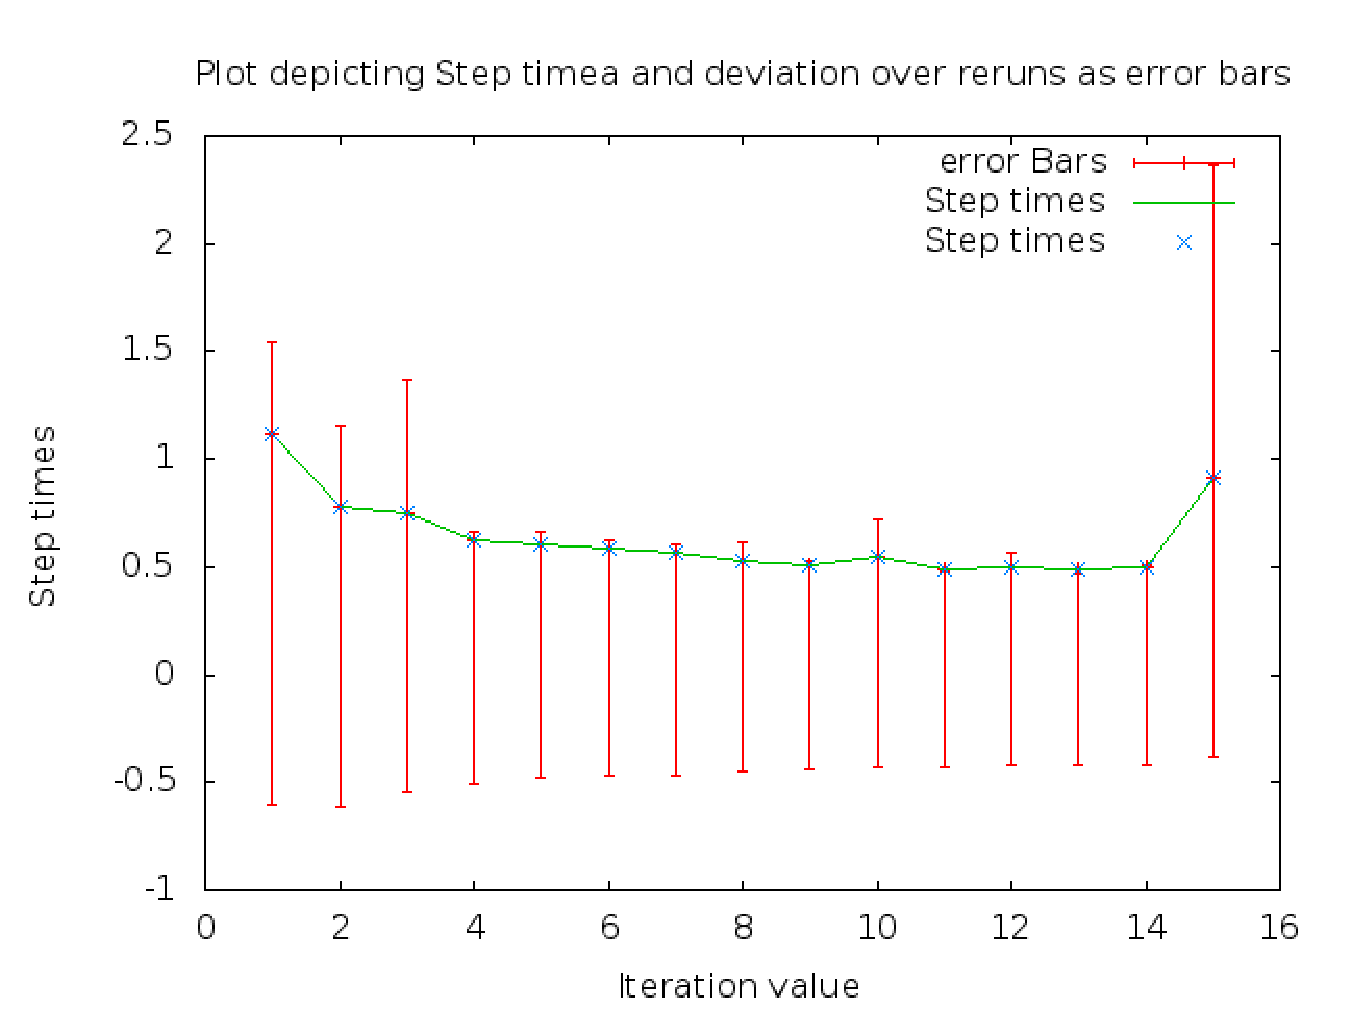
\includegraphics[scale = 0.4]{images/plot3} \\
  \emph{Average step time with error bars v/s iteration value} \\
\end{center}

%%%%%%%%%%%%%%%%%%%%%%%%%%%%%%%%%%%%%%%%%%%%%%%%%%%%%%%%%%%%%%%%%%%%%%%%%%%%%%%%%%%%%%%%%%%

\subsection{Plot4 : Frequency and Cumulative Frequency Plot of Step Time}
\paragraph{}

From the frequency plot of the step time, the most probable step time value (x-axis) 
can be found (by the plot below)
\begin{center}
 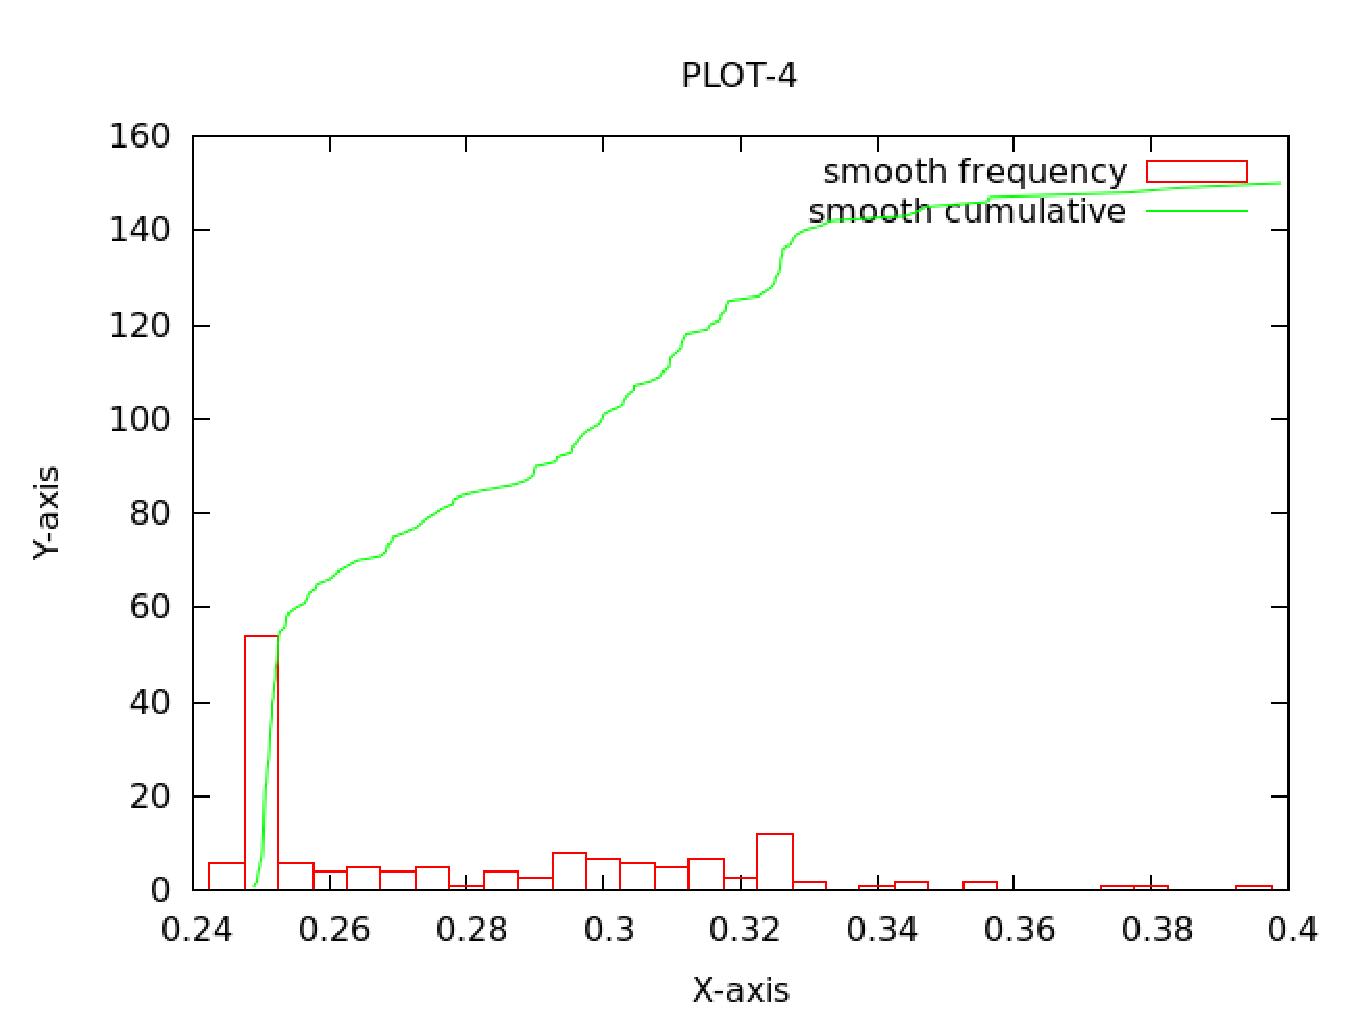
\includegraphics[scale = 0.4]{images/plot4} \\
  \emph{Frequency and Cumulative Frequency Plot of Step Time} \\
\end{center}

%%%%%%%%%%%%%%%%%%%%%%%%%%%%%%%%%%%%%%%%%%%%%%%%%%%%%%%%%%%%%%%%%%%%%%%%%%%%%%%%%%%%%%%%%%%
\subsection{Plot 5 : Best Linear fit for Step Time vs Iteration Value}
\paragraph{}
As the step time varies slightly for all reruns for a particular iteration value thus the random points "x"
and average point "+" become close to each other (with slight deviation in slopes of best fit line).
\begin{center}
 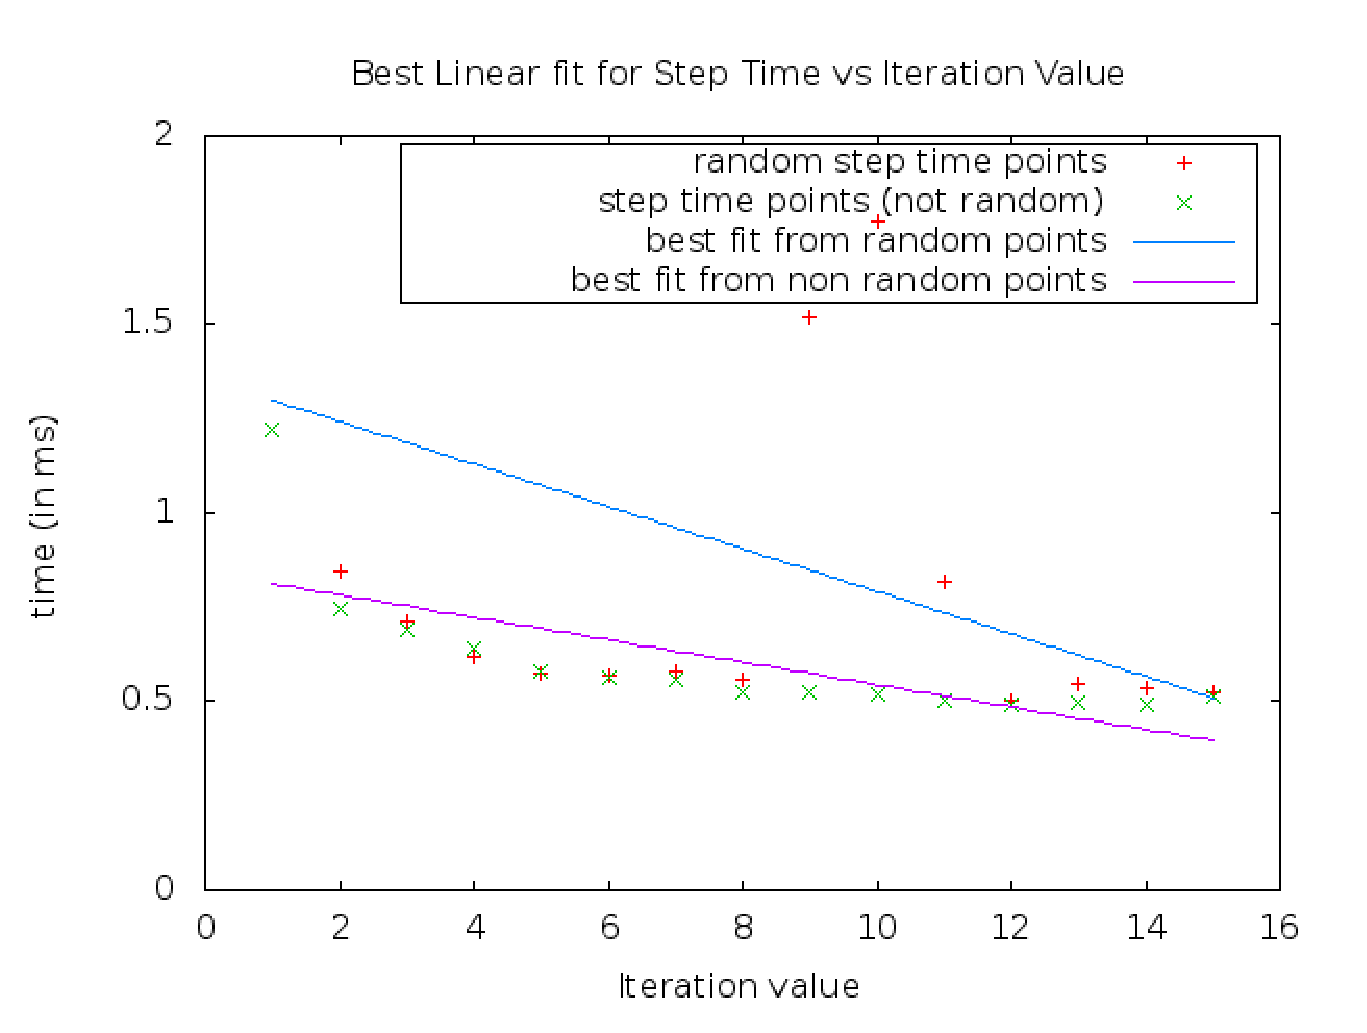
\includegraphics[scale = 0.4]{images/plot5} \\
  \emph{Best Linear fit for Step Time vs Iteration Value} \\
\end{center}

%%%%%%%%%%%%%%%%%%%%%%%%%%%%%%%%%%%%%%%%%%%%%%%%%%%%%%%%%%%%%%%%%%%%%%%%%%%%%%%%%%%%%%%%%%%

\section{Effect of heavy processes}
\paragraph{}

\textit{Heavy processes:-}

As our timing measurement includes other system process time, so by increasing the load on the system by either
 cpu heavy processes like running an application or playing games or by memory heavy processes where a large amount of data
  is being generated or being accessed, loop time and step time can be increased.

\textit{For example,}

Generating all output files (225000) from the executable is a memory heavy process and creating csv from them is a 
cpu heavy process.


\section{Difference between time and gettimeofday}
\paragraph{}

\textbf{Time} command basically gives the complete time for the execution of a process with which it is invoked.
For e.g. while running time with a c++ executable, it will include the time for loading binary files, header files
and the input file given to it.

On the other hand \textbf{gettimeofday} gives the absolute time. Invoking it twice on a piece of code and taking 
the difference between them will give the time system has taken to execute the code between them \textbf{plus} the 
time it used to execute any other system process that was executed between them. It can happen because the system
 can stop executing the code for a while and execute some other process in that time.

\begin{center}
 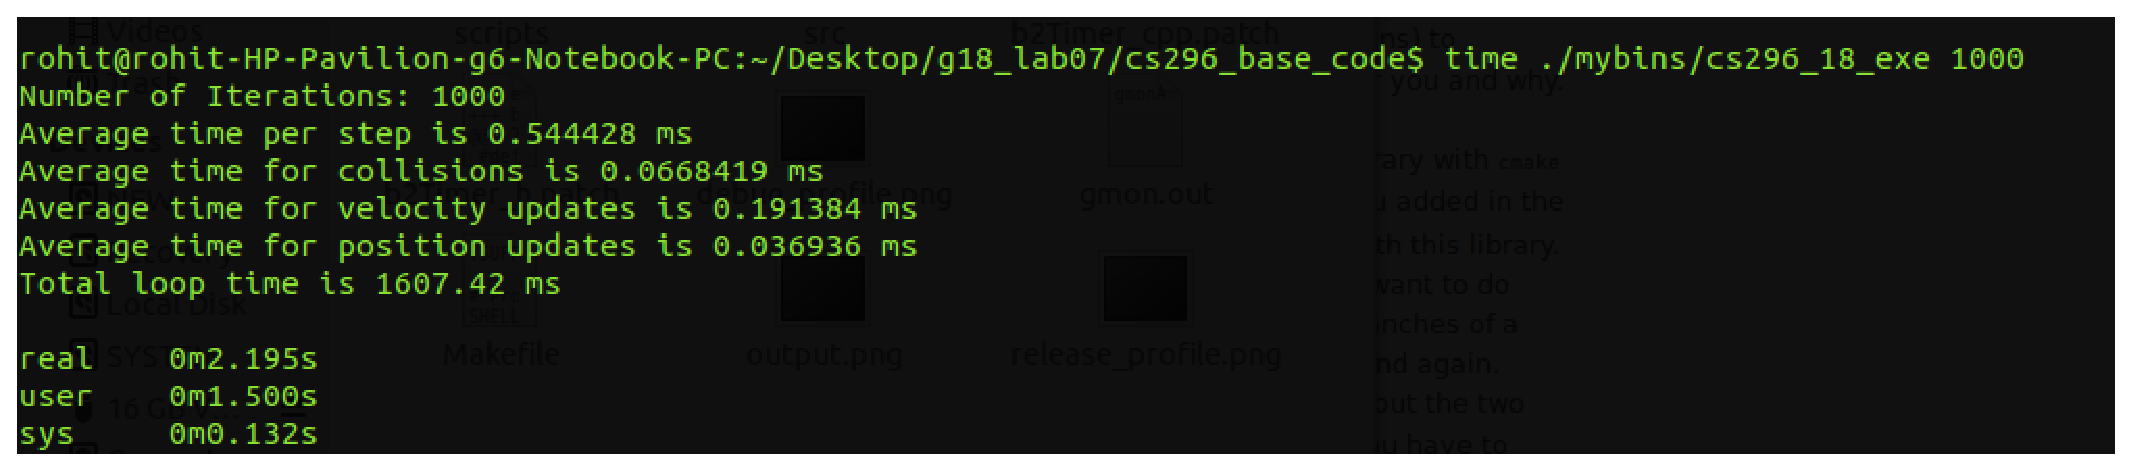
\includegraphics[scale = 0.4]{images/time} \\
  \emph{Time given by time and difference of gettimeofday} \\
\end{center}

The time given by the above process is more by \textit{time} function than\textit{gettimeofday} because
of the time required for loading files (by time) and also, my system was lightly loaded when the above program was executed.


\section{Comparision of release-mode profile and debug-mode profile}
\paragraph{}

Among the used various -On options for optimizing a code using g++ compiler, we have used \textbf{-O3} option 
(for release-mode) to achieve a better optimization level. Although it increases the 
memory requirement for the code significantly, but 
in our case, it didn't mattered a lot. Also, from an analyzing point of view it gives a better perspective on 
how optimization works by the g++ compiler. These include loop unrolling (i.e. an equivalent code without the loop). 
But this increases the size of the code as the same code in the loop is reproduced by the number of times the loop
is going to run.

\subsection{Observations}
\paragraph{}
\textit{Cumulative time comparison:-}


For a iteration value, the cumulative time for debug build type is found to be 5-6 times that for the release build type.
 It was expected as debug would add the debug flags appropriate for your compiler. 
 There are relatively large number of function calls in debug build type,

Ex. for iteration value 10000, debug build time is 0.0592 seconds and release build time is 0.0082 seconds.

\setlength{\parskip}{10pt plus 1pt}
\textit{Function call difference:-}
A set of member functions of ‘b2Vec2’ which includes operators like +, -, and *, b2Cross, b2Mult 
are only executed in debug build type. 

\setlength{\parskip}{10pt plus 1pt}
\textit{Optimization:-}

In the given list of functions, only few functions contribute significant amount of time and a slight difference
 in per-call time of these functions create huge difference in overall performance of both the build type.

For example:- This set of data for iteration value 10000 of the function 
b2World:drawShape, with three functions calls 

\setlength{\parskip}{10pt plus 1pt}

\begin{tabular}{ | l | l | l | l |}
	\hline
  function name  & no of calls & release-mode-time & debug-mode-time \\ \hline
  debug-draw-t::DrawSolidCircle & 1400000 & 0.05 & 0.22 \\ \hline
  debug-draw-t::DrawSolidPolygen & 3100000 & 0.05 & 0.05 \\ \hline
  debug-draw-t::DrawSegment & 100000 & 0.00 & 0.00 \\ \hline
\end{tabular}

\subsection{Call graph using python script}
\paragraph{}
Call graph plots for debug build type is more complex with interlinking among different functions, which explains 
the significant cummulative time difference in debug and release type. 

The call graphs for the debug profile mode have been generated by gprof2dot python 
script. The dot function is used to create a call graph from a DAG (Directed Acyclic Graph)

\begin{lstlisting}
	python scripts/gprof2dot.py ./data/g18_release_prof.dat | dot -Teps -o rls.eps
\end{lstlisting}

The call graphs for the debug profile mode are (splitted into three parts):-

\begin{center}
 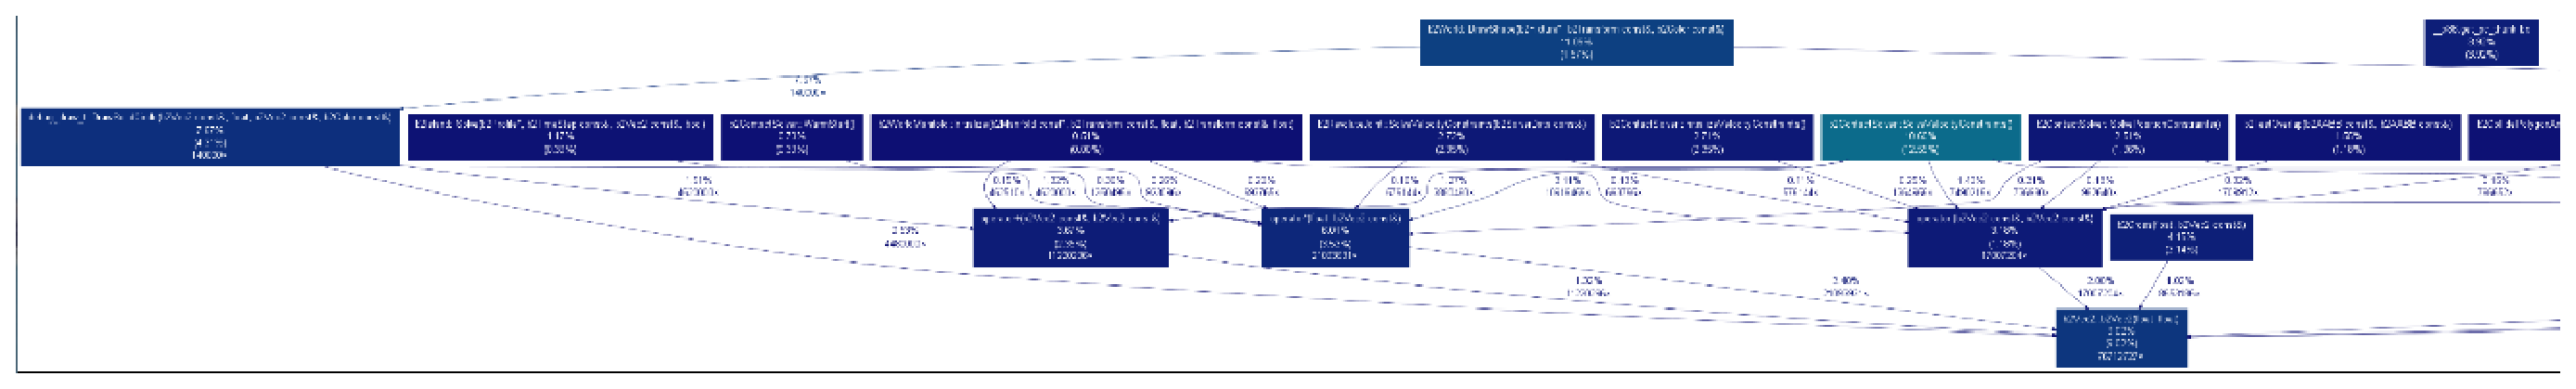
\includegraphics[scale = 0.35]{images/dbg1} \\
\end{center}

\begin{center}
 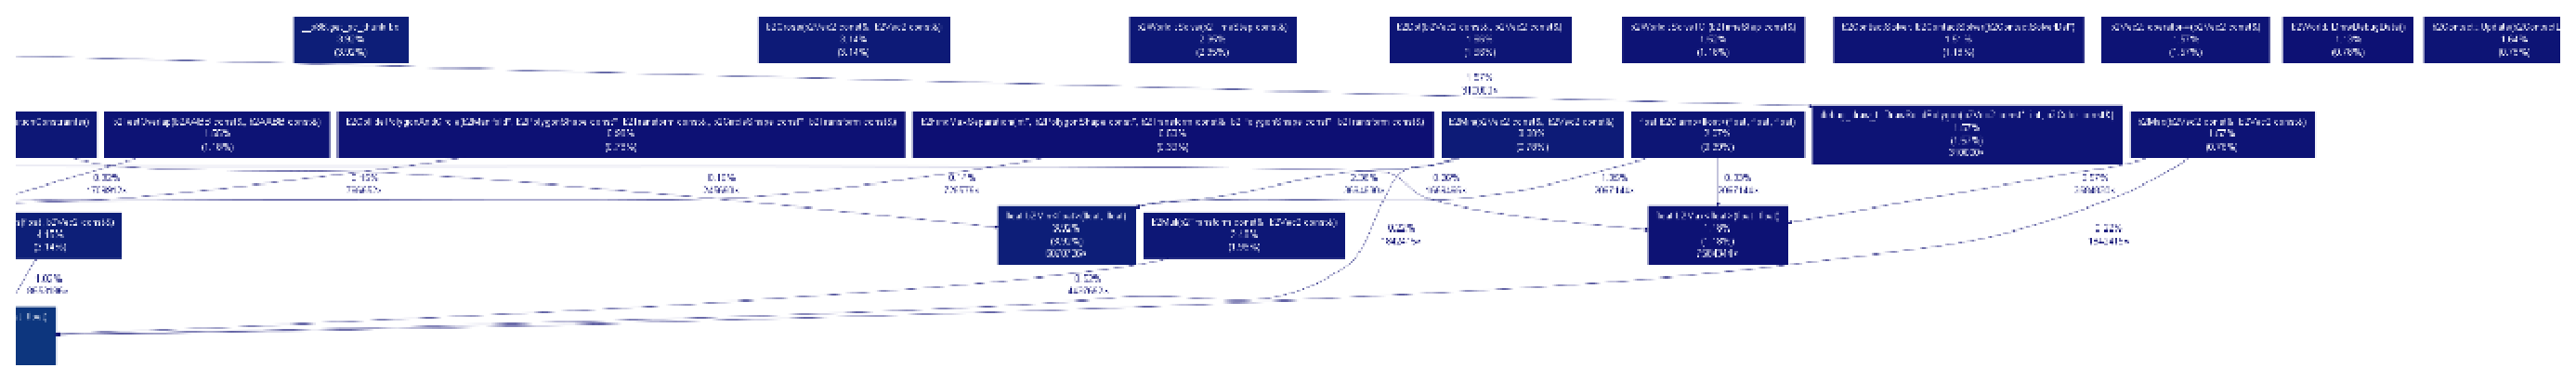
\includegraphics[scale = 0.35]{images/dbg2} \\
\end{center}

\begin{center}
 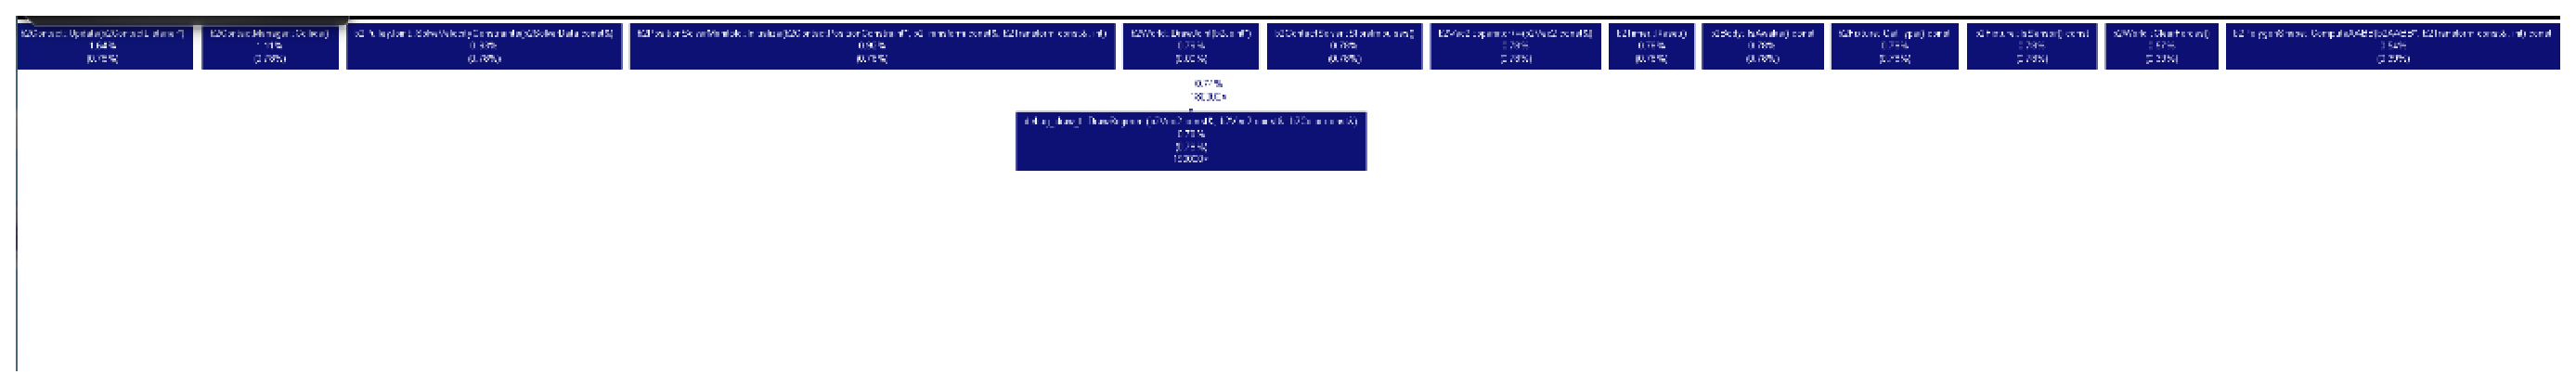
\includegraphics[scale = 0.35]{images/dbg3} \\
\end{center}

The call graphs for the release profile mode are (splitted into three parts):-
\begin{center}
 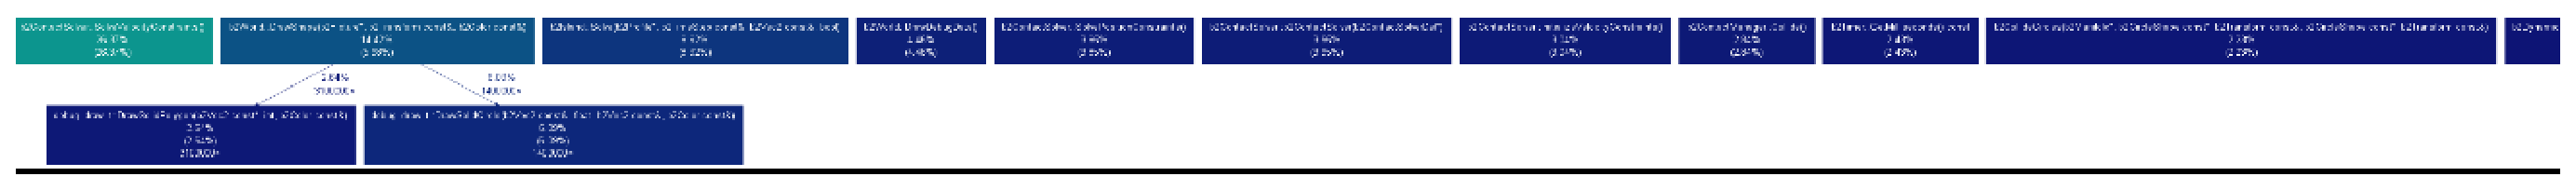
\includegraphics[scale = 0.35]{images/rls1} \\
\end{center}

\begin{center}
 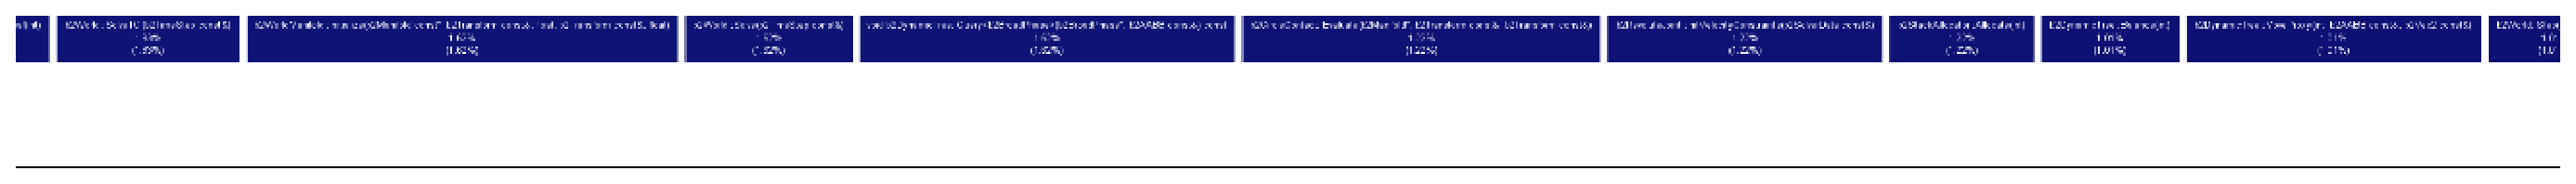
\includegraphics[scale = 0.35]{images/rls2} \\
\end{center}

\begin{center}
 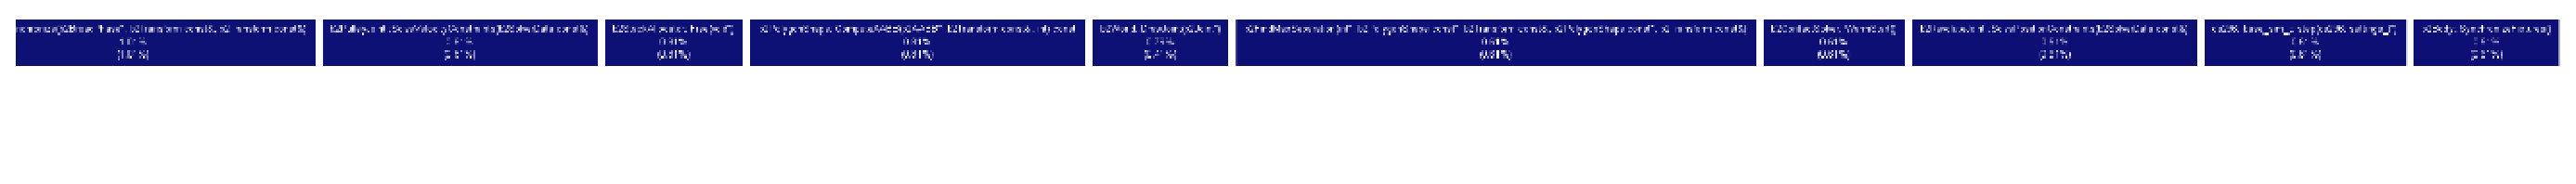
\includegraphics[scale = 0.35]{images/rls3} \\
\end{center}


\section{Conclusions}
\paragraph{}
	We discovered how to get time of particular process using different timers like time, gettimeoftheday and the 
	difference between them. We also learnt to profile code and to analyse time taken by each function call individually 
	and number of calls for a particular function using call graph.

	Further we learnt to create and review call graph plots using python script and then analyze function call complexity graphically
 and learnt comparing each function call time to decide which part of code is required to be optimized.
	
\begin{thebibliography}{1}

\bibitem{gp}
 José Fonseca, https://code.google.com/p/jrfonseca/wiki/Gprof2Dot
 
\end{thebibliography}

\end{document}







